
\section{Ejercicio 3}
\subsection{Introducción}
Contamos con un conjunto de exploradoras a las que se le asigna una letra, cada una con amistades dentro del grupo. 
A partir de esto, buscamos ubicarlas en una ronda que minimice la suma de las distancias entre cada par de amigas.
De esa ronda queremos saber ademas cual fue la distancia máxima entre amigas, y de haber mas de una ronda posible, quedarnos con la primera en orden alfabético.\\
Se pide una complejidad estrictamente mejor que $O(e^ea^2) $, donde $e$ es la cantidad de exploradoras y $a$ la cantidad de amistades.

Por ejemplo:
\\
Se cuenta con las exploradoras  $e = \{a, b, c, d, e\} $  y amistades  $a = \{ (a,b), (a,c), (a,d), (b,e), (c,d) \} $ 

\begin{figure}[H]
  \hspace{-2em}
	\begin{minipage}[h]{0.48\textwidth}
	\begin{center}
		\centering
		  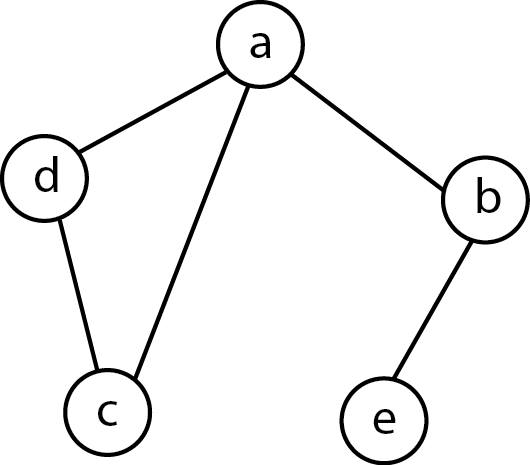
\includegraphics[scale=1]{imagenes/ej3-ejemplo.png}
		 \caption{Ejemplo de configuración óptima}
	\end{center}
	\end{minipage}
	\hspace{3em}
	\begin{minipage}[h]{0.48\textwidth}
	\begin{center}
	   \centering
	       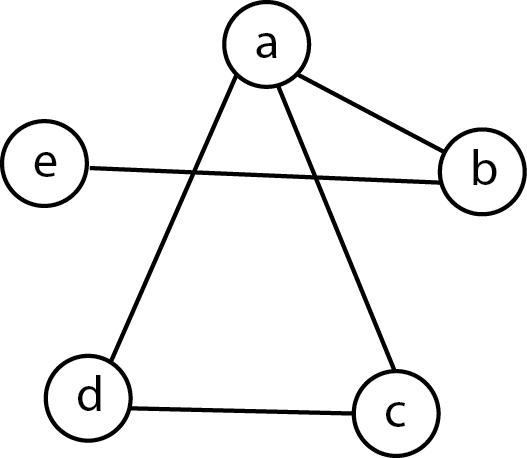
\includegraphics[scale=1]{imagenes/ej3-ejemplo2.png}
	     \caption{Ejemplo de configuración suboptima}
	\end{center}
	\end{minipage}
\end{figure}

La ronda que minimiza la suma de las distancias entre las amistades primera en orden alfabético es $abecd$, donde la distancia para cada amistad es una exploradora, excepto $(a,c)$ que tienen una separación de dos , sumando una distancia total $6$. Para el caso $abcde$, las amistades $(a,b)$ y $(c,d)$ tienen distancia uno, mientras que las demás están separadas por dos, sumando un total de $8$.


\subsection{Desarrollo}
Elegimos utilizar la técnica de backtracking para hallar una solución optima.
A partir de los datos de entrada, construimos una lista de exploradoras en la que guardamos su letra y posición en la ronda. Para indicar que una exploradora no esta en la ronda, utilizamos el indice -1.
Luego definimos una lista de amistades que vincula pares de exploradoras de la lista anterior.
Por último, ordenamos alfabéticamente la lista de exploradoras, para facilitar el orden en que buscaremos soluciones optimas.

Dado que es una estructura circular, siempre podremos ubicar la primer exploradora (por su letra) en la primer posición al representar cualquier ronda optima como una cadena. Al tener la lista de exploradoras ordenada, la primera de la lista estará en el primer lugar a imprimir, por lo que la ubicamos antes de llamar a la función de backtracking. Esto no es estrictamente necesario para la solución, pero elimina una cantidad considerable de operaciones innecesarias.

\newpage

Hecho esto, llamamos a la función recursiva que resuelve el problema.
En cada llamada calculamos primero la suma de las distancias entre las amistades presentes en la ronda. Si esta suma es menor a la mejor solución encontrada, o aun no hallamos una, y faltan exploradoras para completar la ronda, ubicamos cada exploradora posible en la posición actual y llamamos a la recursión indicando que se debe ubicar la siguiente. Si la ronda esta completa, guardamos la suma si es mejor que nuestra solución anterior. Si la suma parcial fue mayor a nuestro candidato a solución óptima, podamos esta rama de decisión para que continúe la recursión de un nivel superior o termine la función.

Al colocar una exploradora en la ronda controlamos primero que no haya sido ubicada previamente. Si no esta presente, le asignamos ademas la posición en que fue colocada. Esto es necesario para que en las sucesivas llamadas recursivas no se intente volver a ubicarla, restringiendo efectivamente el conjunto de exploradoras con el que trabaja cada recursión para que solo pueda colocar las validas.
Una vez terminada la búsqueda por profundidad, se restablece la posición de la exploradora colocada, para que pueda volver a ser utilizada en la próxima llamada recursiva.

Al momento de controlar las distancias, debido al mecanismo detallado en el parrafo anterior, cada exploradora tiene asignada su posición en la ronda. Dada la estructura circular en la que estan dispuestas, con cada exploradora en posiciones numeradas de 0 a la cantidad de exploradoras, la distancia entre cada par puede calcularse como:
 Dadas $a$ y $b$ dos posiciones en la ronda, $a < b$. Sea $t$ el tamaño de la ronda.
Si $b - a > t/2$ entonces la distancia entre $a$ y $b$ es igual a $t+ a - b$.
Sino, la distancia entre $a$ y $b$ es igual a $b - a$.
Esto se debe a que la distancia máxima entre dos puntos de una ronda es la mitad de su tamaño. Si la diferencia entre las posiciones es mayor a este valor, entonces están mas cerca en el sentido contrario. Para ilustrar este caso podemos imaginar que los indices continúan subiendo a medida que terminan los iniciales. Por ejemplo, en una ronda de 5 exploradoras, tras una vuelta de la ronda la exploradora 1 se convierte en la 6, la 2 en la 7, y así sucesivamente. Luego, la distancia entre la exploradora 1 y 5 es igual a la distancia entre la 5 y 6, cuya diferencia de indices es 1.


\subsection{Correctitud}

Podemos garantizar que el resultado obtenido sera una solución optima porque se consideran todas las instancias válidas del problema.
La poda que incorporamos solo elimina casos cuya solución es estrictamente peor que la mejor encontrada. 
Como las distancias entre exploradoras son siempre positivas, la suma parcial de las que ya fueron ubicadas en la ronda es menor o igual a la suma de todas las distancias. Por lo que si esa suma parcial ya es superior a la mejor solución encontrada, cualquier otra configuración de la ronda derivada de esa ronda parcial tendra mayor distancia total.
Al calcular las distancias para cada posible ronda válida y quedarnos con la primer optima encontrada nos aseguramos también de que sea la primera en orden alfabético, ya que recorremos en orden una lista de exploradoras ordenadas por sus letras a medida que generamos las rondas.

\subsection{Complejidad}

Dejando de lado la complejidad de la lectura y construcción de las estructuras a partir de las que se resuelve el problema, incurrimos en una complejidad 
$O(e \ log(e))$ al ordenar la lista de exploradoras.
Para la solución del problema realizamos operaciones de costo constante antes de llamar a la función recursiva. 
Cada llamada a esta función tiene un costo $O(e+a)$ y como no es llamada para exploradoras ya ubicadas, se utiliza $e!$ veces.
Podemos entonces acotar la complejidad de todos los llamados recursivos por $O(e! (e+a))$.\\
Como $e\ log(e) < e! (e+a) $ $\forall{e,a \in \mathbb{N}}$ podemos acotar la complejidad del algoritmo propuesto a $O(e! (e+a))$. 


\subsection{Experimentación}

Para la experimentación consideramos escenarios de peor y mejor caso, así como variaciones en el tamaño de los parámetros de entrada.
Tanto para el peor y mejor caso como para la variación sobre $e$ experimentamos sobre el rango $\#e = 5..12$ para analizar los tiempos de ejecución, que consideramos suficiente a efectos de ilustrar sus relaciones con las cotas de complejidad.

El peor caso para este algoritmo sucede cuando no puede aplicarse ninguna poda, es decir, cuando toda suma parcial de distancias es menor a la distancia óptima.
Esto sucede cuando todas las exploradoras son amigas entre si, formando un grafo completo de amistades. Como la suma de distancias sera igual para toda ronda en esta situación, cualquier suma en rondas incompletas sera menor a la mejor distancia obtenida.
El mejor caso para este algoritmo sucede cuando la configuración óptima es la primera considerada y pueden podarse la mayor cantidad de alternativas.
Por su estructura, en cualquier ronda hay al menos dos configuraciones con distancia optima cuando las distinguimos en algún orden, dado que si se invierte el orden de la mejor ronda se obtiene otra con las mismas distancias. 
Por lo tanto, el mejor caso se da cuando solo estas dos rondas no son podadas.
A partir de esto encontramos que el mejor caso sucede cuando cada exploradora es amiga de la siguiente en orden alfabético, formando un circulo.
\begin{figure}[H]
% GNUPLOT: LaTeX picture
\setlength{\unitlength}{0.240900pt}
\ifx\plotpoint\undefined\newsavebox{\plotpoint}\fi
\begin{picture}(1500,900)(0,0)
\sbox{\plotpoint}{\rule[-0.200pt]{0.400pt}{0.400pt}}%
\put(151.0,131.0){\rule[-0.200pt]{4.818pt}{0.400pt}}
\put(131,131){\makebox(0,0)[r]{ 0}}
\put(1419.0,131.0){\rule[-0.200pt]{4.818pt}{0.400pt}}
\put(151.0,245.0){\rule[-0.200pt]{4.818pt}{0.400pt}}
\put(131,245){\makebox(0,0)[r]{ 5}}
\put(1419.0,245.0){\rule[-0.200pt]{4.818pt}{0.400pt}}
\put(151.0,359.0){\rule[-0.200pt]{4.818pt}{0.400pt}}
\put(131,359){\makebox(0,0)[r]{ 10}}
\put(1419.0,359.0){\rule[-0.200pt]{4.818pt}{0.400pt}}
\put(151.0,472.0){\rule[-0.200pt]{4.818pt}{0.400pt}}
\put(131,472){\makebox(0,0)[r]{ 15}}
\put(1419.0,472.0){\rule[-0.200pt]{4.818pt}{0.400pt}}
\put(151.0,586.0){\rule[-0.200pt]{4.818pt}{0.400pt}}
\put(131,586){\makebox(0,0)[r]{ 20}}
\put(1419.0,586.0){\rule[-0.200pt]{4.818pt}{0.400pt}}
\put(151.0,700.0){\rule[-0.200pt]{4.818pt}{0.400pt}}
\put(131,700){\makebox(0,0)[r]{ 25}}
\put(1419.0,700.0){\rule[-0.200pt]{4.818pt}{0.400pt}}
\put(151.0,814.0){\rule[-0.200pt]{4.818pt}{0.400pt}}
\put(131,814){\makebox(0,0)[r]{ 30}}
\put(1419.0,814.0){\rule[-0.200pt]{4.818pt}{0.400pt}}
\put(151.0,131.0){\rule[-0.200pt]{0.400pt}{4.818pt}}
\put(151,90){\makebox(0,0){ 5}}
\put(151.0,839.0){\rule[-0.200pt]{0.400pt}{4.818pt}}
\put(335.0,131.0){\rule[-0.200pt]{0.400pt}{4.818pt}}
\put(335,90){\makebox(0,0){ 6}}
\put(335.0,839.0){\rule[-0.200pt]{0.400pt}{4.818pt}}
\put(519.0,131.0){\rule[-0.200pt]{0.400pt}{4.818pt}}
\put(519,90){\makebox(0,0){ 7}}
\put(519.0,839.0){\rule[-0.200pt]{0.400pt}{4.818pt}}
\put(703.0,131.0){\rule[-0.200pt]{0.400pt}{4.818pt}}
\put(703,90){\makebox(0,0){ 8}}
\put(703.0,839.0){\rule[-0.200pt]{0.400pt}{4.818pt}}
\put(887.0,131.0){\rule[-0.200pt]{0.400pt}{4.818pt}}
\put(887,90){\makebox(0,0){ 9}}
\put(887.0,839.0){\rule[-0.200pt]{0.400pt}{4.818pt}}
\put(1071.0,131.0){\rule[-0.200pt]{0.400pt}{4.818pt}}
\put(1071,90){\makebox(0,0){ 10}}
\put(1071.0,839.0){\rule[-0.200pt]{0.400pt}{4.818pt}}
\put(1255.0,131.0){\rule[-0.200pt]{0.400pt}{4.818pt}}
\put(1255,90){\makebox(0,0){ 11}}
\put(1255.0,839.0){\rule[-0.200pt]{0.400pt}{4.818pt}}
\put(1439.0,131.0){\rule[-0.200pt]{0.400pt}{4.818pt}}
\put(1439,90){\makebox(0,0){ 12}}
\put(1439.0,839.0){\rule[-0.200pt]{0.400pt}{4.818pt}}
\put(151.0,131.0){\rule[-0.200pt]{0.400pt}{175.375pt}}
\put(151.0,131.0){\rule[-0.200pt]{310.279pt}{0.400pt}}
\put(1439.0,131.0){\rule[-0.200pt]{0.400pt}{175.375pt}}
\put(151.0,859.0){\rule[-0.200pt]{310.279pt}{0.400pt}}
\put(30,495){\makebox(0,0){\rotatebox{90}{Tiempo}}}
\put(795,29){\makebox(0,0){Cantidad de exploradoras}}
\put(1279,819){\makebox(0,0)[r]{Mejor caso}}
\put(1299.0,819.0){\rule[-0.200pt]{24.090pt}{0.400pt}}
\put(151,131){\usebox{\plotpoint}}
\put(593,130.67){\rule{3.132pt}{0.400pt}}
\multiput(593.00,130.17)(6.500,1.000){2}{\rule{1.566pt}{0.400pt}}
\put(151.0,131.0){\rule[-0.200pt]{106.478pt}{0.400pt}}
\put(710,131.67){\rule{3.132pt}{0.400pt}}
\multiput(710.00,131.17)(6.500,1.000){2}{\rule{1.566pt}{0.400pt}}
\put(606.0,132.0){\rule[-0.200pt]{25.054pt}{0.400pt}}
\put(775,132.67){\rule{3.132pt}{0.400pt}}
\multiput(775.00,132.17)(6.500,1.000){2}{\rule{1.566pt}{0.400pt}}
\put(723.0,133.0){\rule[-0.200pt]{12.527pt}{0.400pt}}
\put(828,133.67){\rule{3.132pt}{0.400pt}}
\multiput(828.00,133.17)(6.500,1.000){2}{\rule{1.566pt}{0.400pt}}
\put(788.0,134.0){\rule[-0.200pt]{9.636pt}{0.400pt}}
\put(854,134.67){\rule{3.132pt}{0.400pt}}
\multiput(854.00,134.17)(6.500,1.000){2}{\rule{1.566pt}{0.400pt}}
\put(841.0,135.0){\rule[-0.200pt]{3.132pt}{0.400pt}}
\put(880,135.67){\rule{3.132pt}{0.400pt}}
\multiput(880.00,135.17)(6.500,1.000){2}{\rule{1.566pt}{0.400pt}}
\put(867.0,136.0){\rule[-0.200pt]{3.132pt}{0.400pt}}
\put(906,136.67){\rule{3.132pt}{0.400pt}}
\multiput(906.00,136.17)(6.500,1.000){2}{\rule{1.566pt}{0.400pt}}
\put(893.0,137.0){\rule[-0.200pt]{3.132pt}{0.400pt}}
\put(932,137.67){\rule{3.132pt}{0.400pt}}
\multiput(932.00,137.17)(6.500,1.000){2}{\rule{1.566pt}{0.400pt}}
\put(919.0,138.0){\rule[-0.200pt]{3.132pt}{0.400pt}}
\put(958,138.67){\rule{3.132pt}{0.400pt}}
\multiput(958.00,138.17)(6.500,1.000){2}{\rule{1.566pt}{0.400pt}}
\put(971,139.67){\rule{3.132pt}{0.400pt}}
\multiput(971.00,139.17)(6.500,1.000){2}{\rule{1.566pt}{0.400pt}}
\put(984,140.67){\rule{3.132pt}{0.400pt}}
\multiput(984.00,140.17)(6.500,1.000){2}{\rule{1.566pt}{0.400pt}}
\put(997,141.67){\rule{3.132pt}{0.400pt}}
\multiput(997.00,141.17)(6.500,1.000){2}{\rule{1.566pt}{0.400pt}}
\put(1010,142.67){\rule{3.132pt}{0.400pt}}
\multiput(1010.00,142.17)(6.500,1.000){2}{\rule{1.566pt}{0.400pt}}
\put(1023,143.67){\rule{3.132pt}{0.400pt}}
\multiput(1023.00,143.17)(6.500,1.000){2}{\rule{1.566pt}{0.400pt}}
\put(1036,144.67){\rule{3.132pt}{0.400pt}}
\multiput(1036.00,144.17)(6.500,1.000){2}{\rule{1.566pt}{0.400pt}}
\put(1049,145.67){\rule{3.132pt}{0.400pt}}
\multiput(1049.00,145.17)(6.500,1.000){2}{\rule{1.566pt}{0.400pt}}
\put(1062,146.67){\rule{3.132pt}{0.400pt}}
\multiput(1062.00,146.17)(6.500,1.000){2}{\rule{1.566pt}{0.400pt}}
\put(1075,148.17){\rule{2.700pt}{0.400pt}}
\multiput(1075.00,147.17)(7.396,2.000){2}{\rule{1.350pt}{0.400pt}}
\put(1088,149.67){\rule{3.132pt}{0.400pt}}
\multiput(1088.00,149.17)(6.500,1.000){2}{\rule{1.566pt}{0.400pt}}
\put(1101,151.17){\rule{2.700pt}{0.400pt}}
\multiput(1101.00,150.17)(7.396,2.000){2}{\rule{1.350pt}{0.400pt}}
\put(1114,152.67){\rule{3.132pt}{0.400pt}}
\multiput(1114.00,152.17)(6.500,1.000){2}{\rule{1.566pt}{0.400pt}}
\put(1127,154.17){\rule{2.700pt}{0.400pt}}
\multiput(1127.00,153.17)(7.396,2.000){2}{\rule{1.350pt}{0.400pt}}
\put(1140,156.17){\rule{2.700pt}{0.400pt}}
\multiput(1140.00,155.17)(7.396,2.000){2}{\rule{1.350pt}{0.400pt}}
\put(1153,158.17){\rule{2.700pt}{0.400pt}}
\multiput(1153.00,157.17)(7.396,2.000){2}{\rule{1.350pt}{0.400pt}}
\put(1166,160.17){\rule{2.700pt}{0.400pt}}
\multiput(1166.00,159.17)(7.396,2.000){2}{\rule{1.350pt}{0.400pt}}
\put(1179,162.17){\rule{2.700pt}{0.400pt}}
\multiput(1179.00,161.17)(7.396,2.000){2}{\rule{1.350pt}{0.400pt}}
\multiput(1192.00,164.61)(2.695,0.447){3}{\rule{1.833pt}{0.108pt}}
\multiput(1192.00,163.17)(9.195,3.000){2}{\rule{0.917pt}{0.400pt}}
\put(1205,167.17){\rule{2.700pt}{0.400pt}}
\multiput(1205.00,166.17)(7.396,2.000){2}{\rule{1.350pt}{0.400pt}}
\multiput(1218.00,169.61)(2.695,0.447){3}{\rule{1.833pt}{0.108pt}}
\multiput(1218.00,168.17)(9.195,3.000){2}{\rule{0.917pt}{0.400pt}}
\multiput(1231.00,172.61)(2.695,0.447){3}{\rule{1.833pt}{0.108pt}}
\multiput(1231.00,171.17)(9.195,3.000){2}{\rule{0.917pt}{0.400pt}}
\multiput(1244.00,175.61)(2.695,0.447){3}{\rule{1.833pt}{0.108pt}}
\multiput(1244.00,174.17)(9.195,3.000){2}{\rule{0.917pt}{0.400pt}}
\multiput(1257.00,178.61)(2.695,0.447){3}{\rule{1.833pt}{0.108pt}}
\multiput(1257.00,177.17)(9.195,3.000){2}{\rule{0.917pt}{0.400pt}}
\multiput(1270.00,181.61)(2.695,0.447){3}{\rule{1.833pt}{0.108pt}}
\multiput(1270.00,180.17)(9.195,3.000){2}{\rule{0.917pt}{0.400pt}}
\multiput(1283.00,184.60)(1.797,0.468){5}{\rule{1.400pt}{0.113pt}}
\multiput(1283.00,183.17)(10.094,4.000){2}{\rule{0.700pt}{0.400pt}}
\multiput(1296.00,188.60)(1.797,0.468){5}{\rule{1.400pt}{0.113pt}}
\multiput(1296.00,187.17)(10.094,4.000){2}{\rule{0.700pt}{0.400pt}}
\multiput(1309.00,192.60)(1.797,0.468){5}{\rule{1.400pt}{0.113pt}}
\multiput(1309.00,191.17)(10.094,4.000){2}{\rule{0.700pt}{0.400pt}}
\multiput(1322.00,196.60)(1.797,0.468){5}{\rule{1.400pt}{0.113pt}}
\multiput(1322.00,195.17)(10.094,4.000){2}{\rule{0.700pt}{0.400pt}}
\multiput(1335.00,200.60)(1.797,0.468){5}{\rule{1.400pt}{0.113pt}}
\multiput(1335.00,199.17)(10.094,4.000){2}{\rule{0.700pt}{0.400pt}}
\multiput(1348.00,204.59)(1.378,0.477){7}{\rule{1.140pt}{0.115pt}}
\multiput(1348.00,203.17)(10.634,5.000){2}{\rule{0.570pt}{0.400pt}}
\multiput(1361.00,209.59)(1.378,0.477){7}{\rule{1.140pt}{0.115pt}}
\multiput(1361.00,208.17)(10.634,5.000){2}{\rule{0.570pt}{0.400pt}}
\multiput(1374.00,214.59)(1.378,0.477){7}{\rule{1.140pt}{0.115pt}}
\multiput(1374.00,213.17)(10.634,5.000){2}{\rule{0.570pt}{0.400pt}}
\multiput(1387.00,219.59)(1.378,0.477){7}{\rule{1.140pt}{0.115pt}}
\multiput(1387.00,218.17)(10.634,5.000){2}{\rule{0.570pt}{0.400pt}}
\multiput(1400.00,224.59)(1.123,0.482){9}{\rule{0.967pt}{0.116pt}}
\multiput(1400.00,223.17)(10.994,6.000){2}{\rule{0.483pt}{0.400pt}}
\multiput(1413.00,230.59)(1.123,0.482){9}{\rule{0.967pt}{0.116pt}}
\multiput(1413.00,229.17)(10.994,6.000){2}{\rule{0.483pt}{0.400pt}}
\multiput(1426.00,236.59)(0.950,0.485){11}{\rule{0.843pt}{0.117pt}}
\multiput(1426.00,235.17)(11.251,7.000){2}{\rule{0.421pt}{0.400pt}}
\put(945.0,139.0){\rule[-0.200pt]{3.132pt}{0.400pt}}
\put(1279,778){\makebox(0,0)[r]{Peor caso}}
\multiput(1299,778)(20.756,0.000){5}{\usebox{\plotpoint}}
\put(1399,778){\usebox{\plotpoint}}
\put(151.00,131.00){\usebox{\plotpoint}}
\put(171.76,131.00){\usebox{\plotpoint}}
\put(192.51,131.00){\usebox{\plotpoint}}
\put(213.27,131.00){\usebox{\plotpoint}}
\put(234.02,131.05){\usebox{\plotpoint}}
\put(254.75,132.00){\usebox{\plotpoint}}
\put(275.51,132.00){\usebox{\plotpoint}}
\put(296.26,132.00){\usebox{\plotpoint}}
\put(317.02,132.00){\usebox{\plotpoint}}
\put(337.75,132.76){\usebox{\plotpoint}}
\put(358.50,133.00){\usebox{\plotpoint}}
\put(379.23,134.00){\usebox{\plotpoint}}
\put(399.98,134.23){\usebox{\plotpoint}}
\put(420.70,135.45){\usebox{\plotpoint}}
\put(441.42,136.63){\usebox{\plotpoint}}
\put(462.14,137.83){\usebox{\plotpoint}}
\put(482.86,139.10){\usebox{\plotpoint}}
\put(503.46,141.56){\usebox{\plotpoint}}
\put(524.07,144.07){\usebox{\plotpoint}}
\put(544.67,146.58){\usebox{\plotpoint}}
\put(565.10,150.21){\usebox{\plotpoint}}
\put(585.43,154.36){\usebox{\plotpoint}}
\put(605.57,159.39){\usebox{\plotpoint}}
\put(625.48,165.21){\usebox{\plotpoint}}
\put(645.14,171.86){\usebox{\plotpoint}}
\put(664.33,179.77){\usebox{\plotpoint}}
\put(683.00,188.80){\usebox{\plotpoint}}
\put(701.31,198.57){\usebox{\plotpoint}}
\put(718.40,210.30){\usebox{\plotpoint}}
\put(735.07,222.66){\usebox{\plotpoint}}
\put(751.08,235.86){\usebox{\plotpoint}}
\put(765.99,250.28){\usebox{\plotpoint}}
\put(780.03,265.57){\usebox{\plotpoint}}
\put(793.56,281.30){\usebox{\plotpoint}}
\multiput(805,296)(11.902,17.004){2}{\usebox{\plotpoint}}
\put(829.00,332.42){\usebox{\plotpoint}}
\put(839.38,350.39){\usebox{\plotpoint}}
\multiput(847,364)(9.004,18.701){2}{\usebox{\plotpoint}}
\put(867.26,406.04){\usebox{\plotpoint}}
\multiput(874,420)(8.106,19.107){2}{\usebox{\plotpoint}}
\multiput(888,453)(7.049,19.522){2}{\usebox{\plotpoint}}
\multiput(901,489)(7.013,19.535){2}{\usebox{\plotpoint}}
\multiput(915,528)(6.006,19.867){2}{\usebox{\plotpoint}}
\multiput(928,571)(5.925,19.892){2}{\usebox{\plotpoint}}
\multiput(942,618)(5.127,20.112){3}{\usebox{\plotpoint}}
\multiput(955,669)(5.120,20.114){3}{\usebox{\plotpoint}}
\multiput(969,724)(4.326,20.300){3}{\usebox{\plotpoint}}
\multiput(982,785)(4.070,20.352){3}{\usebox{\plotpoint}}
\put(997,859){\usebox{\plotpoint}}
\sbox{\plotpoint}{\rule[-0.400pt]{0.800pt}{0.800pt}}%
\sbox{\plotpoint}{\rule[-0.200pt]{0.400pt}{0.400pt}}%
\put(1279,737){\makebox(0,0)[r]{$O(e^e)$}}
\sbox{\plotpoint}{\rule[-0.400pt]{0.800pt}{0.800pt}}%
\put(1299.0,737.0){\rule[-0.400pt]{24.090pt}{0.800pt}}
\put(151,132){\usebox{\plotpoint}}
\put(151,130.84){\rule{3.132pt}{0.800pt}}
\multiput(151.00,130.34)(6.500,1.000){2}{\rule{1.566pt}{0.800pt}}
\put(190,131.84){\rule{3.132pt}{0.800pt}}
\multiput(190.00,131.34)(6.500,1.000){2}{\rule{1.566pt}{0.800pt}}
\put(203,132.84){\rule{3.132pt}{0.800pt}}
\multiput(203.00,132.34)(6.500,1.000){2}{\rule{1.566pt}{0.800pt}}
\put(164.0,133.0){\rule[-0.400pt]{6.263pt}{0.800pt}}
\put(229,133.84){\rule{3.132pt}{0.800pt}}
\multiput(229.00,133.34)(6.500,1.000){2}{\rule{1.566pt}{0.800pt}}
\put(242,134.84){\rule{3.132pt}{0.800pt}}
\multiput(242.00,134.34)(6.500,1.000){2}{\rule{1.566pt}{0.800pt}}
\put(255,136.34){\rule{3.132pt}{0.800pt}}
\multiput(255.00,135.34)(6.500,2.000){2}{\rule{1.566pt}{0.800pt}}
\put(268,137.84){\rule{3.132pt}{0.800pt}}
\multiput(268.00,137.34)(6.500,1.000){2}{\rule{1.566pt}{0.800pt}}
\put(281,139.34){\rule{3.132pt}{0.800pt}}
\multiput(281.00,138.34)(6.500,2.000){2}{\rule{1.566pt}{0.800pt}}
\put(294,141.84){\rule{3.132pt}{0.800pt}}
\multiput(294.00,140.34)(6.500,3.000){2}{\rule{1.566pt}{0.800pt}}
\put(307,144.84){\rule{3.132pt}{0.800pt}}
\multiput(307.00,143.34)(6.500,3.000){2}{\rule{1.566pt}{0.800pt}}
\put(320,148.34){\rule{2.800pt}{0.800pt}}
\multiput(320.00,146.34)(7.188,4.000){2}{\rule{1.400pt}{0.800pt}}
\put(333,152.34){\rule{2.800pt}{0.800pt}}
\multiput(333.00,150.34)(7.188,4.000){2}{\rule{1.400pt}{0.800pt}}
\multiput(346.00,157.39)(1.244,0.536){5}{\rule{1.933pt}{0.129pt}}
\multiput(346.00,154.34)(8.987,6.000){2}{\rule{0.967pt}{0.800pt}}
\multiput(359.00,163.39)(1.244,0.536){5}{\rule{1.933pt}{0.129pt}}
\multiput(359.00,160.34)(8.987,6.000){2}{\rule{0.967pt}{0.800pt}}
\multiput(372.00,169.40)(0.737,0.516){11}{\rule{1.356pt}{0.124pt}}
\multiput(372.00,166.34)(10.186,9.000){2}{\rule{0.678pt}{0.800pt}}
\multiput(385.00,178.40)(0.654,0.514){13}{\rule{1.240pt}{0.124pt}}
\multiput(385.00,175.34)(10.426,10.000){2}{\rule{0.620pt}{0.800pt}}
\multiput(398.00,188.41)(0.536,0.511){17}{\rule{1.067pt}{0.123pt}}
\multiput(398.00,185.34)(10.786,12.000){2}{\rule{0.533pt}{0.800pt}}
\multiput(412.41,199.00)(0.509,0.616){19}{\rule{0.123pt}{1.185pt}}
\multiput(409.34,199.00)(13.000,13.541){2}{\rule{0.800pt}{0.592pt}}
\multiput(425.41,215.00)(0.509,0.740){19}{\rule{0.123pt}{1.369pt}}
\multiput(422.34,215.00)(13.000,16.158){2}{\rule{0.800pt}{0.685pt}}
\multiput(438.41,234.00)(0.509,0.905){19}{\rule{0.123pt}{1.615pt}}
\multiput(435.34,234.00)(13.000,19.647){2}{\rule{0.800pt}{0.808pt}}
\multiput(451.41,257.00)(0.509,1.112){19}{\rule{0.123pt}{1.923pt}}
\multiput(448.34,257.00)(13.000,24.009){2}{\rule{0.800pt}{0.962pt}}
\multiput(464.41,285.00)(0.509,1.443){19}{\rule{0.123pt}{2.415pt}}
\multiput(461.34,285.00)(13.000,30.987){2}{\rule{0.800pt}{1.208pt}}
\multiput(477.41,321.00)(0.509,1.733){19}{\rule{0.123pt}{2.846pt}}
\multiput(474.34,321.00)(13.000,37.093){2}{\rule{0.800pt}{1.423pt}}
\multiput(490.41,364.00)(0.509,2.188){19}{\rule{0.123pt}{3.523pt}}
\multiput(487.34,364.00)(13.000,46.688){2}{\rule{0.800pt}{1.762pt}}
\multiput(503.41,418.00)(0.509,2.684){19}{\rule{0.123pt}{4.262pt}}
\multiput(500.34,418.00)(13.000,57.155){2}{\rule{0.800pt}{2.131pt}}
\multiput(516.41,484.00)(0.509,3.346){19}{\rule{0.123pt}{5.246pt}}
\multiput(513.34,484.00)(13.000,71.111){2}{\rule{0.800pt}{2.623pt}}
\multiput(529.41,566.00)(0.509,4.132){19}{\rule{0.123pt}{6.415pt}}
\multiput(526.34,566.00)(13.000,87.685){2}{\rule{0.800pt}{3.208pt}}
\multiput(542.41,667.00)(0.509,5.124){19}{\rule{0.123pt}{7.892pt}}
\multiput(539.34,667.00)(13.000,108.619){2}{\rule{0.800pt}{3.946pt}}
\multiput(555.39,792.00)(0.536,7.272){5}{\rule{0.129pt}{9.133pt}}
\multiput(552.34,792.00)(6.000,48.043){2}{\rule{0.800pt}{4.567pt}}
\put(216.0,135.0){\rule[-0.400pt]{3.132pt}{0.800pt}}
\sbox{\plotpoint}{\rule[-0.200pt]{0.400pt}{0.400pt}}%
\put(151.0,131.0){\rule[-0.200pt]{0.400pt}{175.375pt}}
\put(151.0,131.0){\rule[-0.200pt]{310.279pt}{0.400pt}}
\put(1439.0,131.0){\rule[-0.200pt]{0.400pt}{175.375pt}}
\put(151.0,859.0){\rule[-0.200pt]{310.279pt}{0.400pt}}
\end{picture}

\caption{Comparación de tiempos de mejor y peor caso}
\end{figure}

\newpage

En cuanto a las variaciones del tamaño de entrada, para el primer experimento fijamos la cantidad en un valor arbitrario $\#a = 5$, donde se eligieron amistades sin intencionalidad particular.
\begin{figure}[H]
% GNUPLOT: LaTeX picture
\setlength{\unitlength}{0.240900pt}
\ifx\plotpoint\undefined\newsavebox{\plotpoint}\fi
\sbox{\plotpoint}{\rule[-0.200pt]{0.400pt}{0.400pt}}%
\begin{picture}(1500,900)(0,0)
\sbox{\plotpoint}{\rule[-0.200pt]{0.400pt}{0.400pt}}%
\put(151.0,131.0){\rule[-0.200pt]{4.818pt}{0.400pt}}
\put(131,131){\makebox(0,0)[r]{ 0}}
\put(1419.0,131.0){\rule[-0.200pt]{4.818pt}{0.400pt}}
\put(151.0,245.0){\rule[-0.200pt]{4.818pt}{0.400pt}}
\put(131,245){\makebox(0,0)[r]{ 5}}
\put(1419.0,245.0){\rule[-0.200pt]{4.818pt}{0.400pt}}
\put(151.0,359.0){\rule[-0.200pt]{4.818pt}{0.400pt}}
\put(131,359){\makebox(0,0)[r]{ 10}}
\put(1419.0,359.0){\rule[-0.200pt]{4.818pt}{0.400pt}}
\put(151.0,472.0){\rule[-0.200pt]{4.818pt}{0.400pt}}
\put(131,472){\makebox(0,0)[r]{ 15}}
\put(1419.0,472.0){\rule[-0.200pt]{4.818pt}{0.400pt}}
\put(151.0,586.0){\rule[-0.200pt]{4.818pt}{0.400pt}}
\put(131,586){\makebox(0,0)[r]{ 20}}
\put(1419.0,586.0){\rule[-0.200pt]{4.818pt}{0.400pt}}
\put(151.0,700.0){\rule[-0.200pt]{4.818pt}{0.400pt}}
\put(131,700){\makebox(0,0)[r]{ 25}}
\put(1419.0,700.0){\rule[-0.200pt]{4.818pt}{0.400pt}}
\put(151.0,814.0){\rule[-0.200pt]{4.818pt}{0.400pt}}
\put(131,814){\makebox(0,0)[r]{ 30}}
\put(1419.0,814.0){\rule[-0.200pt]{4.818pt}{0.400pt}}
\put(151.0,131.0){\rule[-0.200pt]{0.400pt}{4.818pt}}
\put(151,90){\makebox(0,0){ 5}}
\put(151.0,839.0){\rule[-0.200pt]{0.400pt}{4.818pt}}
\put(335.0,131.0){\rule[-0.200pt]{0.400pt}{4.818pt}}
\put(335,90){\makebox(0,0){ 6}}
\put(335.0,839.0){\rule[-0.200pt]{0.400pt}{4.818pt}}
\put(519.0,131.0){\rule[-0.200pt]{0.400pt}{4.818pt}}
\put(519,90){\makebox(0,0){ 7}}
\put(519.0,839.0){\rule[-0.200pt]{0.400pt}{4.818pt}}
\put(703.0,131.0){\rule[-0.200pt]{0.400pt}{4.818pt}}
\put(703,90){\makebox(0,0){ 8}}
\put(703.0,839.0){\rule[-0.200pt]{0.400pt}{4.818pt}}
\put(887.0,131.0){\rule[-0.200pt]{0.400pt}{4.818pt}}
\put(887,90){\makebox(0,0){ 9}}
\put(887.0,839.0){\rule[-0.200pt]{0.400pt}{4.818pt}}
\put(1071.0,131.0){\rule[-0.200pt]{0.400pt}{4.818pt}}
\put(1071,90){\makebox(0,0){ 10}}
\put(1071.0,839.0){\rule[-0.200pt]{0.400pt}{4.818pt}}
\put(1255.0,131.0){\rule[-0.200pt]{0.400pt}{4.818pt}}
\put(1255,90){\makebox(0,0){ 11}}
\put(1255.0,839.0){\rule[-0.200pt]{0.400pt}{4.818pt}}
\put(1439.0,131.0){\rule[-0.200pt]{0.400pt}{4.818pt}}
\put(1439,90){\makebox(0,0){ 12}}
\put(1439.0,839.0){\rule[-0.200pt]{0.400pt}{4.818pt}}
\put(151.0,131.0){\rule[-0.200pt]{0.400pt}{175.375pt}}
\put(151.0,131.0){\rule[-0.200pt]{310.279pt}{0.400pt}}
\put(1439.0,131.0){\rule[-0.200pt]{0.400pt}{175.375pt}}
\put(151.0,859.0){\rule[-0.200pt]{310.279pt}{0.400pt}}
\put(30,495){\makebox(0,0){\rotatebox{90}{Tiempo}}}
\put(795,29){\makebox(0,0){Cantidad de exploradoras}}
\put(1279,819){\makebox(0,0)[r]{Resultado experimental}}
\put(1299.0,819.0){\rule[-0.200pt]{24.090pt}{0.400pt}}
\put(151,131){\usebox{\plotpoint}}
\put(437,130.67){\rule{3.132pt}{0.400pt}}
\multiput(437.00,130.17)(6.500,1.000){2}{\rule{1.566pt}{0.400pt}}
\put(151.0,131.0){\rule[-0.200pt]{68.897pt}{0.400pt}}
\put(554,131.67){\rule{3.132pt}{0.400pt}}
\multiput(554.00,131.17)(6.500,1.000){2}{\rule{1.566pt}{0.400pt}}
\put(450.0,132.0){\rule[-0.200pt]{25.054pt}{0.400pt}}
\put(606,132.67){\rule{3.132pt}{0.400pt}}
\multiput(606.00,132.17)(6.500,1.000){2}{\rule{1.566pt}{0.400pt}}
\put(567.0,133.0){\rule[-0.200pt]{9.395pt}{0.400pt}}
\put(645,133.67){\rule{3.132pt}{0.400pt}}
\multiput(645.00,133.17)(6.500,1.000){2}{\rule{1.566pt}{0.400pt}}
\put(619.0,134.0){\rule[-0.200pt]{6.263pt}{0.400pt}}
\put(671,134.67){\rule{3.132pt}{0.400pt}}
\multiput(671.00,134.17)(6.500,1.000){2}{\rule{1.566pt}{0.400pt}}
\put(684,135.67){\rule{3.132pt}{0.400pt}}
\multiput(684.00,135.17)(6.500,1.000){2}{\rule{1.566pt}{0.400pt}}
\put(658.0,135.0){\rule[-0.200pt]{3.132pt}{0.400pt}}
\put(710,136.67){\rule{3.132pt}{0.400pt}}
\multiput(710.00,136.17)(6.500,1.000){2}{\rule{1.566pt}{0.400pt}}
\put(723,137.67){\rule{3.132pt}{0.400pt}}
\multiput(723.00,137.17)(6.500,1.000){2}{\rule{1.566pt}{0.400pt}}
\put(736,138.67){\rule{3.132pt}{0.400pt}}
\multiput(736.00,138.17)(6.500,1.000){2}{\rule{1.566pt}{0.400pt}}
\put(749,139.67){\rule{3.132pt}{0.400pt}}
\multiput(749.00,139.17)(6.500,1.000){2}{\rule{1.566pt}{0.400pt}}
\put(762,140.67){\rule{3.132pt}{0.400pt}}
\multiput(762.00,140.17)(6.500,1.000){2}{\rule{1.566pt}{0.400pt}}
\put(775,141.67){\rule{3.132pt}{0.400pt}}
\multiput(775.00,141.17)(6.500,1.000){2}{\rule{1.566pt}{0.400pt}}
\put(788,142.67){\rule{3.373pt}{0.400pt}}
\multiput(788.00,142.17)(7.000,1.000){2}{\rule{1.686pt}{0.400pt}}
\put(802,144.17){\rule{2.700pt}{0.400pt}}
\multiput(802.00,143.17)(7.396,2.000){2}{\rule{1.350pt}{0.400pt}}
\put(815,146.17){\rule{2.700pt}{0.400pt}}
\multiput(815.00,145.17)(7.396,2.000){2}{\rule{1.350pt}{0.400pt}}
\put(828,147.67){\rule{3.132pt}{0.400pt}}
\multiput(828.00,147.17)(6.500,1.000){2}{\rule{1.566pt}{0.400pt}}
\put(841,149.17){\rule{2.700pt}{0.400pt}}
\multiput(841.00,148.17)(7.396,2.000){2}{\rule{1.350pt}{0.400pt}}
\put(854,151.17){\rule{2.700pt}{0.400pt}}
\multiput(854.00,150.17)(7.396,2.000){2}{\rule{1.350pt}{0.400pt}}
\multiput(867.00,153.61)(2.695,0.447){3}{\rule{1.833pt}{0.108pt}}
\multiput(867.00,152.17)(9.195,3.000){2}{\rule{0.917pt}{0.400pt}}
\put(880,156.17){\rule{2.700pt}{0.400pt}}
\multiput(880.00,155.17)(7.396,2.000){2}{\rule{1.350pt}{0.400pt}}
\multiput(893.00,158.61)(2.695,0.447){3}{\rule{1.833pt}{0.108pt}}
\multiput(893.00,157.17)(9.195,3.000){2}{\rule{0.917pt}{0.400pt}}
\multiput(906.00,161.61)(2.695,0.447){3}{\rule{1.833pt}{0.108pt}}
\multiput(906.00,160.17)(9.195,3.000){2}{\rule{0.917pt}{0.400pt}}
\multiput(919.00,164.61)(2.695,0.447){3}{\rule{1.833pt}{0.108pt}}
\multiput(919.00,163.17)(9.195,3.000){2}{\rule{0.917pt}{0.400pt}}
\multiput(932.00,167.60)(1.797,0.468){5}{\rule{1.400pt}{0.113pt}}
\multiput(932.00,166.17)(10.094,4.000){2}{\rule{0.700pt}{0.400pt}}
\multiput(945.00,171.61)(2.695,0.447){3}{\rule{1.833pt}{0.108pt}}
\multiput(945.00,170.17)(9.195,3.000){2}{\rule{0.917pt}{0.400pt}}
\multiput(958.00,174.59)(1.378,0.477){7}{\rule{1.140pt}{0.115pt}}
\multiput(958.00,173.17)(10.634,5.000){2}{\rule{0.570pt}{0.400pt}}
\multiput(971.00,179.60)(1.797,0.468){5}{\rule{1.400pt}{0.113pt}}
\multiput(971.00,178.17)(10.094,4.000){2}{\rule{0.700pt}{0.400pt}}
\multiput(984.00,183.59)(1.378,0.477){7}{\rule{1.140pt}{0.115pt}}
\multiput(984.00,182.17)(10.634,5.000){2}{\rule{0.570pt}{0.400pt}}
\multiput(997.00,188.59)(1.378,0.477){7}{\rule{1.140pt}{0.115pt}}
\multiput(997.00,187.17)(10.634,5.000){2}{\rule{0.570pt}{0.400pt}}
\multiput(1010.00,193.59)(1.123,0.482){9}{\rule{0.967pt}{0.116pt}}
\multiput(1010.00,192.17)(10.994,6.000){2}{\rule{0.483pt}{0.400pt}}
\multiput(1023.00,199.59)(1.123,0.482){9}{\rule{0.967pt}{0.116pt}}
\multiput(1023.00,198.17)(10.994,6.000){2}{\rule{0.483pt}{0.400pt}}
\multiput(1036.00,205.59)(1.123,0.482){9}{\rule{0.967pt}{0.116pt}}
\multiput(1036.00,204.17)(10.994,6.000){2}{\rule{0.483pt}{0.400pt}}
\multiput(1049.00,211.59)(0.950,0.485){11}{\rule{0.843pt}{0.117pt}}
\multiput(1049.00,210.17)(11.251,7.000){2}{\rule{0.421pt}{0.400pt}}
\multiput(1062.00,218.59)(0.950,0.485){11}{\rule{0.843pt}{0.117pt}}
\multiput(1062.00,217.17)(11.251,7.000){2}{\rule{0.421pt}{0.400pt}}
\multiput(1075.00,225.59)(0.824,0.488){13}{\rule{0.750pt}{0.117pt}}
\multiput(1075.00,224.17)(11.443,8.000){2}{\rule{0.375pt}{0.400pt}}
\multiput(1088.00,233.59)(0.728,0.489){15}{\rule{0.678pt}{0.118pt}}
\multiput(1088.00,232.17)(11.593,9.000){2}{\rule{0.339pt}{0.400pt}}
\multiput(1101.00,242.59)(0.728,0.489){15}{\rule{0.678pt}{0.118pt}}
\multiput(1101.00,241.17)(11.593,9.000){2}{\rule{0.339pt}{0.400pt}}
\multiput(1114.00,251.58)(0.652,0.491){17}{\rule{0.620pt}{0.118pt}}
\multiput(1114.00,250.17)(11.713,10.000){2}{\rule{0.310pt}{0.400pt}}
\multiput(1127.00,261.58)(0.590,0.492){19}{\rule{0.573pt}{0.118pt}}
\multiput(1127.00,260.17)(11.811,11.000){2}{\rule{0.286pt}{0.400pt}}
\multiput(1140.00,272.58)(0.590,0.492){19}{\rule{0.573pt}{0.118pt}}
\multiput(1140.00,271.17)(11.811,11.000){2}{\rule{0.286pt}{0.400pt}}
\multiput(1153.00,283.58)(0.539,0.492){21}{\rule{0.533pt}{0.119pt}}
\multiput(1153.00,282.17)(11.893,12.000){2}{\rule{0.267pt}{0.400pt}}
\multiput(1166.00,295.58)(0.497,0.493){23}{\rule{0.500pt}{0.119pt}}
\multiput(1166.00,294.17)(11.962,13.000){2}{\rule{0.250pt}{0.400pt}}
\multiput(1179.58,308.00)(0.493,0.536){23}{\rule{0.119pt}{0.531pt}}
\multiput(1178.17,308.00)(13.000,12.898){2}{\rule{0.400pt}{0.265pt}}
\multiput(1192.58,322.00)(0.493,0.536){23}{\rule{0.119pt}{0.531pt}}
\multiput(1191.17,322.00)(13.000,12.898){2}{\rule{0.400pt}{0.265pt}}
\multiput(1205.58,336.00)(0.493,0.616){23}{\rule{0.119pt}{0.592pt}}
\multiput(1204.17,336.00)(13.000,14.771){2}{\rule{0.400pt}{0.296pt}}
\multiput(1218.58,352.00)(0.493,0.616){23}{\rule{0.119pt}{0.592pt}}
\multiput(1217.17,352.00)(13.000,14.771){2}{\rule{0.400pt}{0.296pt}}
\multiput(1231.58,368.00)(0.493,0.695){23}{\rule{0.119pt}{0.654pt}}
\multiput(1230.17,368.00)(13.000,16.643){2}{\rule{0.400pt}{0.327pt}}
\multiput(1244.58,386.00)(0.493,0.734){23}{\rule{0.119pt}{0.685pt}}
\multiput(1243.17,386.00)(13.000,17.579){2}{\rule{0.400pt}{0.342pt}}
\multiput(1257.58,405.00)(0.493,0.774){23}{\rule{0.119pt}{0.715pt}}
\multiput(1256.17,405.00)(13.000,18.515){2}{\rule{0.400pt}{0.358pt}}
\multiput(1270.58,425.00)(0.493,0.814){23}{\rule{0.119pt}{0.746pt}}
\multiput(1269.17,425.00)(13.000,19.451){2}{\rule{0.400pt}{0.373pt}}
\multiput(1283.58,446.00)(0.493,0.853){23}{\rule{0.119pt}{0.777pt}}
\multiput(1282.17,446.00)(13.000,20.387){2}{\rule{0.400pt}{0.388pt}}
\multiput(1296.58,468.00)(0.493,0.933){23}{\rule{0.119pt}{0.838pt}}
\multiput(1295.17,468.00)(13.000,22.260){2}{\rule{0.400pt}{0.419pt}}
\multiput(1309.58,492.00)(0.493,0.972){23}{\rule{0.119pt}{0.869pt}}
\multiput(1308.17,492.00)(13.000,23.196){2}{\rule{0.400pt}{0.435pt}}
\multiput(1322.58,517.00)(0.493,1.052){23}{\rule{0.119pt}{0.931pt}}
\multiput(1321.17,517.00)(13.000,25.068){2}{\rule{0.400pt}{0.465pt}}
\multiput(1335.58,544.00)(0.493,1.091){23}{\rule{0.119pt}{0.962pt}}
\multiput(1334.17,544.00)(13.000,26.004){2}{\rule{0.400pt}{0.481pt}}
\multiput(1348.58,572.00)(0.493,1.171){23}{\rule{0.119pt}{1.023pt}}
\multiput(1347.17,572.00)(13.000,27.877){2}{\rule{0.400pt}{0.512pt}}
\multiput(1361.58,602.00)(0.493,1.250){23}{\rule{0.119pt}{1.085pt}}
\multiput(1360.17,602.00)(13.000,29.749){2}{\rule{0.400pt}{0.542pt}}
\multiput(1374.58,634.00)(0.493,1.290){23}{\rule{0.119pt}{1.115pt}}
\multiput(1373.17,634.00)(13.000,30.685){2}{\rule{0.400pt}{0.558pt}}
\multiput(1387.58,667.00)(0.493,1.408){23}{\rule{0.119pt}{1.208pt}}
\multiput(1386.17,667.00)(13.000,33.493){2}{\rule{0.400pt}{0.604pt}}
\multiput(1400.58,703.00)(0.493,1.448){23}{\rule{0.119pt}{1.238pt}}
\multiput(1399.17,703.00)(13.000,34.430){2}{\rule{0.400pt}{0.619pt}}
\multiput(1413.58,740.00)(0.493,1.567){23}{\rule{0.119pt}{1.331pt}}
\multiput(1412.17,740.00)(13.000,37.238){2}{\rule{0.400pt}{0.665pt}}
\multiput(1426.58,780.00)(0.493,1.607){23}{\rule{0.119pt}{1.362pt}}
\multiput(1425.17,780.00)(13.000,38.174){2}{\rule{0.400pt}{0.681pt}}
\put(697.0,137.0){\rule[-0.200pt]{3.132pt}{0.400pt}}
\put(1279,778){\makebox(0,0)[r]{$O(e^e)$}}
\multiput(1299,778)(20.756,0.000){5}{\usebox{\plotpoint}}
\put(1399,778){\usebox{\plotpoint}}
\put(151,132){\usebox{\plotpoint}}
\put(151.00,132.00){\usebox{\plotpoint}}
\put(171.72,133.00){\usebox{\plotpoint}}
\put(192.47,133.19){\usebox{\plotpoint}}
\put(213.16,134.78){\usebox{\plotpoint}}
\put(233.89,135.38){\usebox{\plotpoint}}
\put(254.59,136.97){\usebox{\plotpoint}}
\put(275.17,139.55){\usebox{\plotpoint}}
\put(295.71,142.39){\usebox{\plotpoint}}
\put(315.93,147.06){\usebox{\plotpoint}}
\put(335.85,152.88){\usebox{\plotpoint}}
\put(355.20,160.25){\usebox{\plotpoint}}
\put(373.85,169.28){\usebox{\plotpoint}}
\put(390.70,181.39){\usebox{\plotpoint}}
\put(406.49,194.83){\usebox{\plotpoint}}
\put(420.22,210.34){\usebox{\plotpoint}}
\put(432.33,227.18){\usebox{\plotpoint}}
\put(443.14,244.87){\usebox{\plotpoint}}
\multiput(450,257)(8.740,18.825){2}{\usebox{\plotpoint}}
\multiput(463,285)(7.049,19.522){2}{\usebox{\plotpoint}}
\multiput(476,321)(6.006,19.867){2}{\usebox{\plotpoint}}
\multiput(489,364)(4.858,20.179){2}{\usebox{\plotpoint}}
\multiput(502,418)(4.011,20.364){4}{\usebox{\plotpoint}}
\multiput(515,484)(3.250,20.499){4}{\usebox{\plotpoint}}
\multiput(528,566)(2.650,20.586){4}{\usebox{\plotpoint}}
\multiput(541,667)(2.147,20.644){7}{\usebox{\plotpoint}}
\multiput(554,792)(1.851,20.673){3}{\usebox{\plotpoint}}
\put(560,859){\usebox{\plotpoint}}
\put(151.0,131.0){\rule[-0.200pt]{0.400pt}{175.375pt}}
\put(151.0,131.0){\rule[-0.200pt]{310.279pt}{0.400pt}}
\put(1439.0,131.0){\rule[-0.200pt]{0.400pt}{175.375pt}}
\put(151.0,859.0){\rule[-0.200pt]{310.279pt}{0.400pt}}
\end{picture}

\caption{Comparación de tiempos sobre variaciones de $e$}
\end{figure}

En el segundo experimento consideramos variaciones de $\#a$ entre 5 y 40, a incrementos de 5, con una cantidad de exploradoras fija $\#e = 7$ que permite analizar este rango de amistades rápidamente. Dado que fijamos $e$, comparamos los resultados obtenidos con la complejidad lineal sobre $a$.

\begin{figure}[H]
% GNUPLOT: LaTeX picture
\setlength{\unitlength}{0.240900pt}
\ifx\plotpoint\undefined\newsavebox{\plotpoint}\fi
\begin{picture}(1500,900)(0,0)
\sbox{\plotpoint}{\rule[-0.200pt]{0.400pt}{0.400pt}}%
\put(191.0,131.0){\rule[-0.200pt]{4.818pt}{0.400pt}}
\put(171,131){\makebox(0,0)[r]{ 0}}
\put(1419.0,131.0){\rule[-0.200pt]{4.818pt}{0.400pt}}
\put(191.0,277.0){\rule[-0.200pt]{4.818pt}{0.400pt}}
\put(171,277){\makebox(0,0)[r]{ 0.02}}
\put(1419.0,277.0){\rule[-0.200pt]{4.818pt}{0.400pt}}
\put(191.0,422.0){\rule[-0.200pt]{4.818pt}{0.400pt}}
\put(171,422){\makebox(0,0)[r]{ 0.04}}
\put(1419.0,422.0){\rule[-0.200pt]{4.818pt}{0.400pt}}
\put(191.0,568.0){\rule[-0.200pt]{4.818pt}{0.400pt}}
\put(171,568){\makebox(0,0)[r]{ 0.06}}
\put(1419.0,568.0){\rule[-0.200pt]{4.818pt}{0.400pt}}
\put(191.0,713.0){\rule[-0.200pt]{4.818pt}{0.400pt}}
\put(171,713){\makebox(0,0)[r]{ 0.08}}
\put(1419.0,713.0){\rule[-0.200pt]{4.818pt}{0.400pt}}
\put(191.0,859.0){\rule[-0.200pt]{4.818pt}{0.400pt}}
\put(171,859){\makebox(0,0)[r]{ 0.1}}
\put(1419.0,859.0){\rule[-0.200pt]{4.818pt}{0.400pt}}
\put(191.0,131.0){\rule[-0.200pt]{0.400pt}{4.818pt}}
\put(191,90){\makebox(0,0){ 5}}
\put(191.0,839.0){\rule[-0.200pt]{0.400pt}{4.818pt}}
\put(369.0,131.0){\rule[-0.200pt]{0.400pt}{4.818pt}}
\put(369,90){\makebox(0,0){ 10}}
\put(369.0,839.0){\rule[-0.200pt]{0.400pt}{4.818pt}}
\put(548.0,131.0){\rule[-0.200pt]{0.400pt}{4.818pt}}
\put(548,90){\makebox(0,0){ 15}}
\put(548.0,839.0){\rule[-0.200pt]{0.400pt}{4.818pt}}
\put(726.0,131.0){\rule[-0.200pt]{0.400pt}{4.818pt}}
\put(726,90){\makebox(0,0){ 20}}
\put(726.0,839.0){\rule[-0.200pt]{0.400pt}{4.818pt}}
\put(904.0,131.0){\rule[-0.200pt]{0.400pt}{4.818pt}}
\put(904,90){\makebox(0,0){ 25}}
\put(904.0,839.0){\rule[-0.200pt]{0.400pt}{4.818pt}}
\put(1082.0,131.0){\rule[-0.200pt]{0.400pt}{4.818pt}}
\put(1082,90){\makebox(0,0){ 30}}
\put(1082.0,839.0){\rule[-0.200pt]{0.400pt}{4.818pt}}
\put(1261.0,131.0){\rule[-0.200pt]{0.400pt}{4.818pt}}
\put(1261,90){\makebox(0,0){ 35}}
\put(1261.0,839.0){\rule[-0.200pt]{0.400pt}{4.818pt}}
\put(1439.0,131.0){\rule[-0.200pt]{0.400pt}{4.818pt}}
\put(1439,90){\makebox(0,0){ 40}}
\put(1439.0,839.0){\rule[-0.200pt]{0.400pt}{4.818pt}}
\put(191.0,131.0){\rule[-0.200pt]{0.400pt}{175.375pt}}
\put(191.0,131.0){\rule[-0.200pt]{300.643pt}{0.400pt}}
\put(1439.0,131.0){\rule[-0.200pt]{0.400pt}{175.375pt}}
\put(191.0,859.0){\rule[-0.200pt]{300.643pt}{0.400pt}}
\put(30,495){\makebox(0,0){\rotatebox{90}{Tiempo}}}
\put(815,29){\makebox(0,0){Cantidad amistades}}
\put(1279,819){\makebox(0,0)[r]{Resultado experimental}}
\put(1299.0,819.0){\rule[-0.200pt]{24.090pt}{0.400pt}}
\put(191,146){\usebox{\plotpoint}}
\put(304,145.67){\rule{3.132pt}{0.400pt}}
\multiput(304.00,145.17)(6.500,1.000){2}{\rule{1.566pt}{0.400pt}}
\put(191.0,146.0){\rule[-0.200pt]{27.222pt}{0.400pt}}
\put(367,146.67){\rule{3.132pt}{0.400pt}}
\multiput(367.00,146.17)(6.500,1.000){2}{\rule{1.566pt}{0.400pt}}
\put(317.0,147.0){\rule[-0.200pt]{12.045pt}{0.400pt}}
\put(431,147.67){\rule{2.891pt}{0.400pt}}
\multiput(431.00,147.17)(6.000,1.000){2}{\rule{1.445pt}{0.400pt}}
\put(380.0,148.0){\rule[-0.200pt]{12.286pt}{0.400pt}}
\put(494,148.67){\rule{2.891pt}{0.400pt}}
\multiput(494.00,148.17)(6.000,1.000){2}{\rule{1.445pt}{0.400pt}}
\put(443.0,149.0){\rule[-0.200pt]{12.286pt}{0.400pt}}
\put(557,149.67){\rule{2.891pt}{0.400pt}}
\multiput(557.00,149.17)(6.000,1.000){2}{\rule{1.445pt}{0.400pt}}
\put(506.0,150.0){\rule[-0.200pt]{12.286pt}{0.400pt}}
\put(645,150.67){\rule{2.891pt}{0.400pt}}
\multiput(645.00,150.17)(6.000,1.000){2}{\rule{1.445pt}{0.400pt}}
\put(569.0,151.0){\rule[-0.200pt]{18.308pt}{0.400pt}}
\put(771,151.67){\rule{2.891pt}{0.400pt}}
\multiput(771.00,151.17)(6.000,1.000){2}{\rule{1.445pt}{0.400pt}}
\put(657.0,152.0){\rule[-0.200pt]{27.463pt}{0.400pt}}
\put(897,152.67){\rule{3.132pt}{0.400pt}}
\multiput(897.00,152.17)(6.500,1.000){2}{\rule{1.566pt}{0.400pt}}
\put(783.0,153.0){\rule[-0.200pt]{27.463pt}{0.400pt}}
\put(998,153.67){\rule{2.891pt}{0.400pt}}
\multiput(998.00,153.17)(6.000,1.000){2}{\rule{1.445pt}{0.400pt}}
\put(910.0,154.0){\rule[-0.200pt]{21.199pt}{0.400pt}}
\put(1086,154.67){\rule{3.132pt}{0.400pt}}
\multiput(1086.00,154.17)(6.500,1.000){2}{\rule{1.566pt}{0.400pt}}
\put(1010.0,155.0){\rule[-0.200pt]{18.308pt}{0.400pt}}
\put(1149,155.67){\rule{3.132pt}{0.400pt}}
\multiput(1149.00,155.17)(6.500,1.000){2}{\rule{1.566pt}{0.400pt}}
\put(1099.0,156.0){\rule[-0.200pt]{12.045pt}{0.400pt}}
\put(1212,156.67){\rule{3.132pt}{0.400pt}}
\multiput(1212.00,156.17)(6.500,1.000){2}{\rule{1.566pt}{0.400pt}}
\put(1162.0,157.0){\rule[-0.200pt]{12.045pt}{0.400pt}}
\put(1275,157.67){\rule{3.132pt}{0.400pt}}
\multiput(1275.00,157.17)(6.500,1.000){2}{\rule{1.566pt}{0.400pt}}
\put(1225.0,158.0){\rule[-0.200pt]{12.045pt}{0.400pt}}
\put(1338,158.67){\rule{3.132pt}{0.400pt}}
\multiput(1338.00,158.17)(6.500,1.000){2}{\rule{1.566pt}{0.400pt}}
\put(1288.0,159.0){\rule[-0.200pt]{12.045pt}{0.400pt}}
\put(1351.0,160.0){\rule[-0.200pt]{21.199pt}{0.400pt}}
\put(1279,778){\makebox(0,0)[r]{O(a)}}
\multiput(1299,778)(20.756,0.000){5}{\usebox{\plotpoint}}
\put(1399,778){\usebox{\plotpoint}}
\put(191,167){\usebox{\plotpoint}}
\put(191.00,167.00){\usebox{\plotpoint}}
\put(211.19,171.80){\usebox{\plotpoint}}
\put(231.57,175.64){\usebox{\plotpoint}}
\put(251.90,179.68){\usebox{\plotpoint}}
\put(272.22,183.87){\usebox{\plotpoint}}
\put(292.53,188.13){\usebox{\plotpoint}}
\put(312.82,192.36){\usebox{\plotpoint}}
\put(333.15,196.52){\usebox{\plotpoint}}
\put(353.48,200.65){\usebox{\plotpoint}}
\put(373.85,204.58){\usebox{\plotpoint}}
\put(394.09,209.18){\usebox{\plotpoint}}
\put(414.44,213.18){\usebox{\plotpoint}}
\put(434.83,216.96){\usebox{\plotpoint}}
\put(455.19,220.88){\usebox{\plotpoint}}
\put(475.38,225.70){\usebox{\plotpoint}}
\put(495.78,229.44){\usebox{\plotpoint}}
\put(516.10,233.55){\usebox{\plotpoint}}
\put(536.39,237.83){\usebox{\plotpoint}}
\put(556.72,241.94){\usebox{\plotpoint}}
\put(577.00,246.23){\usebox{\plotpoint}}
\put(597.29,250.51){\usebox{\plotpoint}}
\put(617.65,254.46){\usebox{\plotpoint}}
\put(638.02,258.39){\usebox{\plotpoint}}
\put(658.21,263.19){\usebox{\plotpoint}}
\put(678.60,266.99){\usebox{\plotpoint}}
\put(698.97,270.92){\usebox{\plotpoint}}
\put(719.33,274.89){\usebox{\plotpoint}}
\put(739.57,279.52){\usebox{\plotpoint}}
\put(759.94,283.45){\usebox{\plotpoint}}
\put(780.27,287.55){\usebox{\plotpoint}}
\put(800.53,292.05){\usebox{\plotpoint}}
\put(820.90,295.98){\usebox{\plotpoint}}
\put(841.23,300.11){\usebox{\plotpoint}}
\put(861.52,304.39){\usebox{\plotpoint}}
\put(881.84,308.46){\usebox{\plotpoint}}
\put(902.13,312.79){\usebox{\plotpoint}}
\put(922.42,317.06){\usebox{\plotpoint}}
\put(942.79,320.95){\usebox{\plotpoint}}
\put(963.18,324.73){\usebox{\plotpoint}}
\put(983.36,329.59){\usebox{\plotpoint}}
\put(1003.73,333.43){\usebox{\plotpoint}}
\put(1024.11,337.26){\usebox{\plotpoint}}
\put(1044.44,341.41){\usebox{\plotpoint}}
\put(1064.69,345.92){\usebox{\plotpoint}}
\put(1085.05,349.85){\usebox{\plotpoint}}
\put(1105.36,354.06){\usebox{\plotpoint}}
\put(1125.68,358.28){\usebox{\plotpoint}}
\put(1146.03,362.31){\usebox{\plotpoint}}
\put(1166.30,366.72){\usebox{\plotpoint}}
\put(1186.62,370.91){\usebox{\plotpoint}}
\put(1206.99,374.84){\usebox{\plotpoint}}
\put(1227.39,378.60){\usebox{\plotpoint}}
\put(1247.57,383.44){\usebox{\plotpoint}}
\put(1267.95,387.24){\usebox{\plotpoint}}
\put(1288.33,391.08){\usebox{\plotpoint}}
\put(1308.63,395.33){\usebox{\plotpoint}}
\put(1328.90,399.72){\usebox{\plotpoint}}
\put(1349.24,403.73){\usebox{\plotpoint}}
\put(1369.53,408.00){\usebox{\plotpoint}}
\put(1389.86,412.14){\usebox{\plotpoint}}
\put(1410.22,416.13){\usebox{\plotpoint}}
\put(1430.45,420.68){\usebox{\plotpoint}}
\put(1439,422){\usebox{\plotpoint}}
\put(191.0,131.0){\rule[-0.200pt]{0.400pt}{175.375pt}}
\put(191.0,131.0){\rule[-0.200pt]{300.643pt}{0.400pt}}
\put(1439.0,131.0){\rule[-0.200pt]{0.400pt}{175.375pt}}
\put(191.0,859.0){\rule[-0.200pt]{300.643pt}{0.400pt}}
\end{picture}

\caption{Comparación de tiempos sobre variaciones de $a$}
\end{figure}







